\chapter{Programming Interface for {\MPI}}

   This chapter describes the programming interface for {\MPI},
   which are widely used for parallel programming for cluster computing.
   Users can introduce {\MPI} functions to {\XMP} using the interface.   

   {\XMP} provides the following user API functions to mix {\MPI}
   functions with {\XMP}.

\begin{itemize}
\item {\tt xmp\_get\_mpi\_comm}
\item {\tt xmp\_init\_mpi}
\item {\tt xmp\_finalize\_mpi}
\end{itemize}

\section{\tt xmp\_get\_mpi\_comm}
\index{xmp\_get\_mpi\_comm@{\tt xmp\_get\_mpi\_comm}}

\subsubsection*{Format}

\begin{tabular}{lll}
\verb![F]!&  {\tt integer function}& {\tt xmp\_get\_mpi\_comm()}\\
\verb![C]!&  {\tt MPI\_Comm}& {\tt xmp\_get\_mpi\_comm(void)}
\end{tabular}

\subsubsection*{Synopsis}

   {\tt xmp\_get\_mpi\_comm} returns the handle of the communicator
   associated with the executing node set. 

\subsubsection*{Arguments}

none.

\section{\tt xmp\_init\_mpi}
\index{xmp\_init\_mpi@{\tt xmp\_init\_mpi}}

\subsubsection*{Format}

\begin{tabular}{lll}
\verb![F]!&  {\tt }& {\tt xmp\_init\_mpi()}\\

\verb![C]!&  {\tt void}& {\tt xmp\_init\_mpi(int *argc, char ***argv)}
\end{tabular}

\subsubsection*{Synopsis}

   {\tt xmp\_init\_mpi} initializes the MPI execution environment.

\subsubsection*{Arguments}

   In {\XMPC}, the command-line arguments {\tt argc} and {\tt argv}
   should be given to {\tt xmp\_init\_mpi}.


\section{\tt xmp\_finalize\_mpi}
\index{xmp\_finalize\_mpi@{\tt xmp\_finalize\_mpi}}

\subsubsection*{Format}

\begin{tabular}{lll}
\verb![F]!&  {\tt }& {\tt xmp\_finalize\_mpi()}\\

\verb![C]!&  {\tt void}& {\tt xmp\_finalize\_mpi(void)}
\end{tabular}

\subsubsection*{Synopsis}

   {\tt xmp\_finalize\_mpi} terminates the MPI execution environment.

\subsubsection*{Arguments}

   none.

\section*{Example}
\index{Example!MPI interface}

\begin{XCexample}
#include <stdio.h>
#include "mpi.h"
#include "xmp.h"

#pragma xmp nodes p[4]

int main(int argc, char *argv[]) {
  xmp_init_mpi(&argc, &argv)

  int rank, size;
  MPI_Comm_rank(MPI_COMM_WORLD, &rank);
  MPI_Comm_size(MPI_COMM_WORLD, &size);

#pragma xmp task on p[1:2]
{
  MPI_Comm comm = xmp_get_mpi_comm(); // get the MPI communicator of p[1:2]

  int rank, size;
  MPI_Comm_rank(comm, &rank);
  MPI_Comm_size(comm, &size);
}

  xmp_finalize_mpi();

  return 0;
}
\end{XCexample}

\cleardoublepage

% \chapter{Directive for Thread Parallelism}
% \index{Directive!threads clause@{\tt threads} clause}

% Thread-level parallelism is needed to program multi-core cluster system.
% Users can use some features introduced from {\OMP} to parallelize loops
% in thread level with the {\tt threads} clause of the {\tt loop}
% directive. No direct use of {\OMP} directives in {\XMP} code is
% allowed.

% \section{{\tt threads} clause}
% \index{threads clause@{\tt threads} clause}

% \subsection*{Syntax}
% \Syntax{loop}

% \begin{tabular}{ll}
% \verb![F]! & \verb|!$xmp| {\tt loop} {\openb} \verb|(| {\it loop-index}
%  {\openb}, {\it loop-index}{\closeb}... \verb|)| {\closeb} \\
%  & \hspace{3cm}{\tt on} \{{\it nodes-ref} $\vert$ {\it template-ref}\}
%      {\openb} {\it reduction-clause} {\closeb}...
%      {\openb} {\it threads-clause} {\closeb} \\
%  & {\it do-loops} \\
%  & \\
% \verb![C]! & \verb|#pragma xmp| {\tt loop} {\openb} \verb|(| {\it
%      loop-index} {\openb}, {\it loop-index}{\closeb}... \verb|)|
%      {\closeb} \\
%  & \hspace{3cm}{\tt on} \{{\it nodes-ref} $\vert$ {\it template-ref}\}
%      {\openb} {\it reduction-clause} {\closeb}...
%      {\openb} {\it threads-clause} {\closeb} \\
%  & {\it for-loops} \\
% \end{tabular}

% \vspace{0.3cm}

% where {\it threads-clause} is:

% \vspace{0.3cm}

% \begin{tabular}{ll}
%  & {\tt threads} {\openb} {\it omp-clause} {\closeb} \\
% \end{tabular}

% \vspace{0.3cm}

% and {\it omp-clause} is one of:

% \vspace{0.3cm}

% \begin{tabular}{ll}
%  & {\tt num\_threads(} {\it num-thread} {\tt )}\\
%  & {\tt private(} {\it list} {\tt )}\\
%  & {\tt firstprivate(} {\it list} {\tt )}\\
%  & {\tt lastprivate(} {\it list} {\tt )}\\
% \end{tabular}

% \subsection*{Description}

%    {\OMP} clauses such as {\tt num\_threads} can be specified in {\tt
%    threads} clause.
%    The {\XMP} compiler generates internally {\OMP} directives from the
%    {\tt loop} directive and the {\tt threads} clause.
%    Note that no {\tt reduction} need to be specified in the {\tt
%    threads} clause because it is inherited from the {\tt reduction}
%    clause in the {\tt loop} directive.

% \subsection*{Example}
% \index{Example!OpenMP interface}

%    This example calculates the total sum of an array.
%    A {\tt threads} clause is given to the {\tt loop} directive to
%    parallelize the loop statement in both process and
%    thread level. 
%    The {\tt reduction} clause in the {\tt loop} directive is also
%    applied to the {\OMP} directive which is generated by the {\XMP}
%    compiler.

% \begin{XCexample}
% #include <stdio.h>
% #include "xmp.h"
% #define N 1024

% #pragma xmp nodes p(*)
% #pragma xmp template t(0:N-1)
% #pragma xmp distribute t(block) onto p
% #pragma xmp align a[i] with t(i)

% int main(void) {
%   . . . // initialize a[]

%   int sum = 0;
% #pragma xmp loop on t(i) reduction(+:sum) threads num_threads(4)
%   for (int i = 0; i < N; i++) {
%     sum += a[i];
%   }

%   return 0;
% }
% \end{XCexample}

% \cleardoublepage


\chapter{Interface to Numerical Libraries}
\label{chap:Interface to Numerical Libraries}
\index{library interface}

   This chapter describes the XcalableMP interfaces to existing MPI
   parallel libraries, which is effective to achieve high productivity
   and performance of {\XMP} programs.
   
\section{Design of the Interface}

A recommended design of the interface is as follows:

\begin{itemize}

 \item Numerical library routines can be invoked by an {\XMP} procedure
       through an interface procedure (Figure \ref{figb.1}).

 \begin{myfigure}
  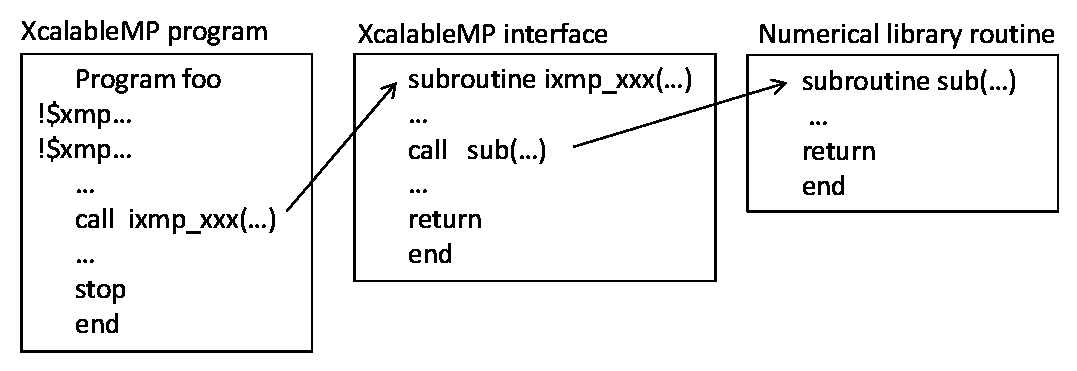
\includegraphics[scale=0.45]{figs/figb.1.eps}
  \caption{Invocation of a Library Routine through an Interface Procedure}
  \label{figb.1}
 \end{myfigure}

 \item When the numerical library routine needs information on an global
       array, the interface extracts it from the descriptor using some
       query routines provided by {\XMP} and passes it to the
       numerical library routine as arguments.
%
 \item The interface does not affect the behavior of numerical library
       routines except for restrictions concerning the {\XMP}
       specification.
\end{itemize}


\section{Extended Mapping Inquiry Functions}

In this section, the extended mapping inquiry functions, which are
implementation-dependent, are shown.
Specifications of the functions below are from the Omni XcalableMP
compiler (\url{http://www.xcalablemp.org/download.html}).

\subsection{\tt xmp\_array\_gtol} \label{subsec:xmparraygtol}
\Intrinsic{xmp\_array\_gtol}

\begin{tabular}{lll}

\verb![F]!& {\tt integer function} & {\tt xmp\_array\_gtol(d, dim, g\_idx, l\_idx)} \\
          & {\tt type(xmp\_desc)} & {\tt d}\\
          & {\tt integer} & {\tt dim}\\
          & {\tt integer} & {\tt g\_idx}\\
          & {\tt integer} & {\tt l\_idx}\\
          & & \\
\verb![C]!&  {\tt void} & {\tt xmp\_array\_gtol(xmp\_desc\_t d, int dim, int g\_idx, int* l\_idx)}

\end{tabular}

\subsubsection*{Synopsis}

The {\tt xmp\_array\_gtol} function translates a global index specified by {\tt g\_idx} of a global array specified by {\tt d} into the corresponding index of its local section and sets to an array specified by {\tt l\_idx}. 
If the element of the specified index does not reside in the caller of the function, 
the resulting array is set to an unspecified value.

\subsubsection*{Input Arguments}

\begin{itemize}
 \item {\tt d} is a descriptor of the global array.
 \item {\tt dim} is the target dimension of the global array.
 \item {\tt g\_idx} is an index of the global array.
\end{itemize}

\subsubsection*{Output Argument}

\begin{itemize}
 \item {\tt l\_idx} is an index of the local array.
\end{itemize}

\subsection{\tt xmp\_array\_lsize}\label{subsec:xmparraylsize}
\index{xmp\_array\_lsize@{\tt xmp\_array\_lsize}}

\subsubsection*{Format}

\begin{tabular}{lll}

\verb![F]!& {\tt integer function}& {\tt xmp\_array\_lsize(d, dim, lsize)}\\
          & {\tt type(xmp\_desc)} & {\tt d}\\
          & {\tt integer} & {\tt dim}\\
          & {\tt integer} & {\tt lsize}\\

\verb![C]!&  {\tt int}& {\tt xmp\_array\_lsize(xmp\_desc\_t d, int dim, int *lsize)}\\

\end{tabular}

\subsubsection*{Synopsis}

The {\tt xmp\_array\_lsize} function provides the local size of each
dimension of the target global array. 
Note that the local size does not include the size of the shadow.

\subsubsection*{Input Arguments}
\begin{itemize}
 \item {\tt d} is a descriptor of a global array.
 \item {\tt dim} is the target dimension of the global array.
\end{itemize}

\subsubsection*{Output Argument}
\begin{itemize}
 \item {\tt lsize} is the local size of the target dimension of the global array.
\end{itemize}


\subsection{\tt xmp\_array\_laddr}
\index{xmp\_array\_laddr@{\tt xmp\_array\_laddr}}

\subsubsection*{Format}

\begin{tabular}{lll}

\verb![C]!&  {\tt int}& {\tt xmp\_array\_laddr(xmp\_desc\_t d, void **laddr)}\\

\end{tabular}

\subsubsection*{Synopsis}

The {\tt xmp\_array\_laddr} function provides the local address of the
target global array. 

\subsubsection*{Input Arguments}
\begin{itemize}
 \item {\tt d} is a descriptor of a global array.
\end{itemize}

\subsubsection*{Output Arguments}
\begin{itemize}
 \item {\tt laddr} is the local address of the target global array.
\end{itemize}


\subsection{\tt xmp\_array\_lda}\label{subsec:xmparraylda}

\subsubsection*{Format}
\begin{tabular}{lll}
\verb![F]!& {\tt integer function}& {\tt xmp\_array\_lda(d, lda)}\\
          & {\tt type(xmp\_desc)} & {\tt d}\\
          & {\tt integer} & {\tt lda}\\
\verb![C]!&  {\tt int}& {\tt xmp\_array\_lda(xmp\_desc\_t d, int* lda)}\\
\end{tabular}

\subsubsection*{Synopsis}
The {\tt xmp\_array\_lda} function provides the leading dimension of the two-dimensional global array.
This function is used to call numerical libraries, such as BLAS.

\subsubsection*{Input Argument}
\begin{itemize}
 \item {\tt d} is a descriptor of a global array which must be a two-dimensional array.
\end{itemize}

\subsubsection*{Output Argument}
\begin{itemize}
 \item {\tt lda} is a leading dimesion of the target global array.
\end{itemize}


\section{Example}
\index{Example!library interface}

   This section shows the interface to ScaLAPACK as an example of the
   {\XMP} interface to numerical libraries.
   
   ScaLAPACK is a linear algebra library for distributed-memory.
   Communication processes in the ScaLAPACK routines depends on BLACS
   (Basic Linear Algebraic Communication Subprograms).
   ScaLAPACK library routines invoked from {\XMP} procedures also depend
   on BLACS. %Remarks of the design of the interface are as follows.

%\begin{itemize}
%\item For a ScaLAPACK library routine having a descriptor array as an
%      argument, the interface procedure has the BLACS context handle
%      including the descriptor array as an additional argument.
%\item The {\tt blacs\_exit} routine is unnecessary because an {\XMP}
%      program executes {\tt MPI\_Finalize}.
%\item Only ``column-major'' is effective as the argument ``order'' of a
%      BLACS routine {\tt blacs\_gridinit}.
%\end{itemize}

\begin{description}

 \item[Example 1]
	    This example shows an implementation of the interface for
	    the ScaLAPACK driver routine {\tt pdgesv}.

\begin{XFexample}
      subroutine ixmp_pdgesv(n,nrhs,a,ia,ja,da,ipiv,b,ib,jb,db,ictxt,info)

      use xmp_lib

      integer n,nrhs,ia,ja,ib,jb,ictxt,info,desca(9),descb(9),ierr
      double precision a,b
      type(xmp_desc) da,db,dta,dtb
      integer lbound_a1,ubound_a1,lbound_a2,ubound_a2
      integer blocksize_a1,blocksize_a2,lead_dim_a
      integer lbound_b1,ubound_b1,lbound_b2,ubound_b2
      integer blocksize_b1,blocksize_b2,lead_dim_b
      
      ierr=xmp_array_lbound(da,1,lbound_a1)
      ierr=xmp_array_ubound(da,1,ubound_a1)
      ierr=xmp_array_lbound(da,2,lbound_a2)
      ierr=xmp_array_ubound(da,2,ubound_a2)
      ierr=xmp_align_template(da,dta)
      ierr=xmp_dist_blocksize(dta,1,blocksize_a1)
      ierr=xmp_dist_blocksize(dta,2,blocksize_a2)
      ierr=xmp_array_lead_dim(da,1,lead_dim_a)
      
      ierr=xmp_array_lbound(db,1,lbound_b1)
      ierr=xmp_array_ubound(db,1,ubound_b1)
      ierr=xmp_array_lbound(db,2,lbound_b2)
      ierr=xmp_array_ubound(db,2,ubound_b2)
      ierr=xmp_align_template(db,dtb)
      ierr=xmp_dist_blocksize(dtb,1,blocksize_b1)
      ierr=xmp_dist_blocksize(dtb,2,blocksize_b2)
      ierr=xmp_array_lead_dim(db,1,lead_dim_b)
      
      desca(1)=1
      desca(2)=ictxt
      desca(3)=ubound_a1-lbound_a1+1
      desca(4)=ubound_a2-lbound_a2+1
      desca(5)=blocksize_a1
      desca(6)=blocksize_a2
      desca(7)=0
      desca(8)=0
      desca(9)=lead_dim_a
      
      descb(1)=1
      descb(2)=ictxt
      descb(3)=ubound_b1-lbound_b1+1
      descb(4)=ubound_b2-lbound_b2+1
      descb(5)=blocksize_b1
      descb(6)=blocksize_b2
      descb(7)=0
      descb(8)=0
      descb(9)=lead_dim_b
      
      call pdgesv(n,nhrs,a,ia,ja,desca,ipiv,b,ib,jb,descb,info)
      
      return
      end

\end{XFexample}


\item[Example 2]
	   This example shows an {\XMP} procedure using the interface of
	   Example 1.

\Example{nodes}
\Example{template}
\Example{distribute}
\Example{align}
\Example{loop}
\begin{XFexample}
      program xmptdgesv

      use xmp_lib

      double precision a(1000,1000)
      double precision b(1000)
      integer ipiv(2*1000,2)
!$xmp nodes p(2,2)
!$xmp template t(1000,1000)
!$xmp template t1(2*1000,2)
!$xmp distribute t(block,block) onto p
!$xmp distribute t1(block,block) onto p
!$xmp align a(i,j) with t(i,j)
!$xmp align ipiv(i,j) with t1(i,j)
!$xmp align b(i) with t(i,*)
      ...
      integer i,j,ictxt
      integer m=1000,n=1000,nprow=2,npcol=2
      integer icontxt=-1,iwhat=0
      integer nrhs=1,ia=1,ja=1,ib=1,jb=1,info
      character*1 order
      ...
      order="C"
      ...
      call blacs_get(icontxt,iwhat,ictxt)
      call blacs_gridinit(ictxt,order,nprow,npcol)
      ...
!$xmp loop (i,j) on t(i,j)
      do j=1,n
         do i=1,m
            a(i,j) = ...
         end do
      end do
      ...
!$xmp loop on t(i,*)
      do i=1,m
         b(i)= ...
      end do
      ...
      call ixmp_pdgesv(n,nrhs,a,ia,ja,xmp_desc_of(a),ipiv,
     *                b,ib,jb,xmp_desc_of(b),ictxt,info)
      ...
      call blacs_gridexit(ictxt)
      ...
      stop
      end
\end{XFexample}
\end{description}


\chapter{Memory-layout Model}

In this chapter, the memory-layout model of global data in the Omni
{\XMP} compiler (\url{http://www.xcalablemp.org/download.html}) is
presented for reference.

The {\XMP} specification says that a global array is distributed onto
a node array according to the data-mapping directives and, as a
result, a node owns a set of elements.

On each node, all and only the elements of the global array that it
owns are gathered to form the local array of the same rank as the
global. For each axis of the global data, all and only the indices 
that the node owns are packed to the axis of the local array so that
sequence can be maintained, with shadow area, if any, added at the
lower and/or upper bound of the axis.

Eventually the local array is stored in memory on each node according
to the rule for storing arrays in the base language, that is, in
row-major order in XMP/Fortran and in column-major order in XMP/C.

Note that, as a result of the model above, memory usage can be
non-uniform among the nodes.

\subsubsection*{Example}
\Example{memory-layout}

\begin{XFexample}
!$xmp nodes p(4,4)
!$xmp template t(64,64)
!$xmp distribute t(block,block) onto p

      real a(64,64)
!$xmp align a(i,j) with t(i,j)
!$xmp shadow a(1,1)
\end{XFexample}

The array {\tt a} is distributed by a format of {\tt (block,block)} onto
a two-dimensional node array {\tt p} and each node owns a local array
including a shadow area. Then the local array is stored in memory on
each node as shown in Figure \ref{figc.1}.

\begin{myfigure}
 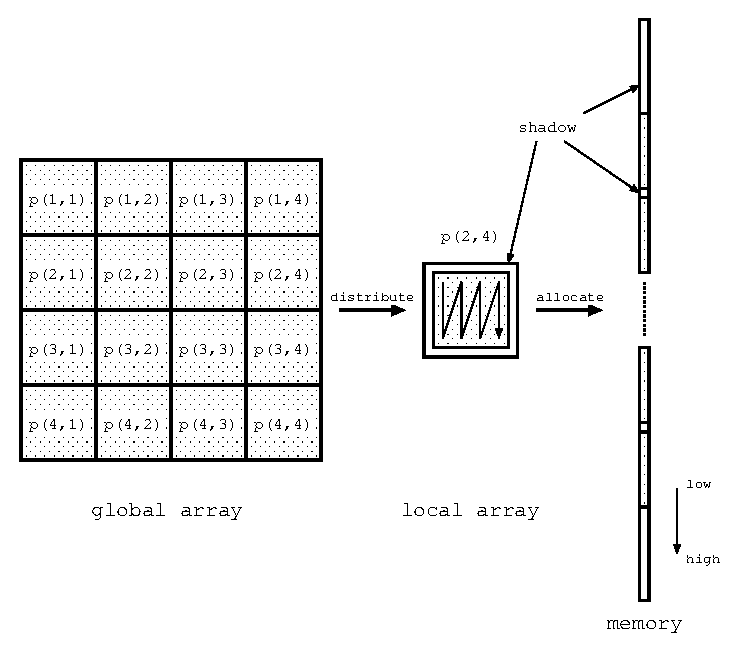
\includegraphics[scale=0.9]{figs/figc.1.eps}
 \caption{Example of Memory Layout in the Omni {\XMP} compiler}
 \label{figc.1}
\end{myfigure}
